

\subsection{Karhunen-Loève Expansion of Functionals}



Assume that $Y \in L^2([0,T]) \cap \Lambda_T$ has  zero mean (otherwise, see \cref{rem:center}).   \cref{thm:KL} suggests to set  $\frakF$  equal to the eigenfunctions of  $\kappa_Y(s,t) = (y_s,y_t)_{L^2(\Q)}$. Optimality comes, however,  at the cost of explicitizing $\frakF$. We proceed as follows: take a regular partition $\Pi_N = \{t_n = n\, \delta t\, |\, n=0,\ldots,N\}$, $ \delta t =\frac{T}{N}$ and compute the kernel matrix $\kappa^{N}_Y = (\kappa_Y(t_n,t_m))_{0 \le n,m \le N}$. When $\kappa_Y$ does not admit a  closed-form expression, $\kappa^{N}_Y$ is replaced by the sample covariance matrix using simulated paths for $Y$. The eigenfunctions thus become eigenvectors and solve the systems\footnote{In  $\eqref{eq:eigendecomp}$,  $\sum"$ means that the first and last summand are halved, i.e. the trapezoidal rule is used to compute  $(\kappa_Y(\cdot,t), F_k)$. Another approach, known as Nyström's method  \cite{reinhardt} consists of   employing a Gaussian quadrature scheme instead.  
However, for large $N$,  we haven't observed any improvement 
and thus favor the more convenient discretization in  $\eqref{eq:eigendecomp}$.}
\vspace{-1mm}
\begin{equation}\label{eq:eigendecomp}
        \sum_{t_n\in  \Pi_N}\!\!" \, \kappa^{N}_{Y}(t_n,t_m) F_{k}(t_n)  \delta t = \lambda^{\frakF}_{k}\,  F_{k}(t_m), \quad t_m\in \Pi_N, \quad k=0,...,N.
\end{equation}
\vspace{-3mm}

 This is a simple eigenvalue problem so  all pairs $(F_k,\lambda_k^{\frakF})$ can be  computed in one go. Let us proceed with two examples where  $T=1$ and $\Q=$ Wiener measure throughout.

\begin{figure}[t]
    \centering
    \caption{Running maximum functional for two trajectories.}
    \vspace{-2mm}
    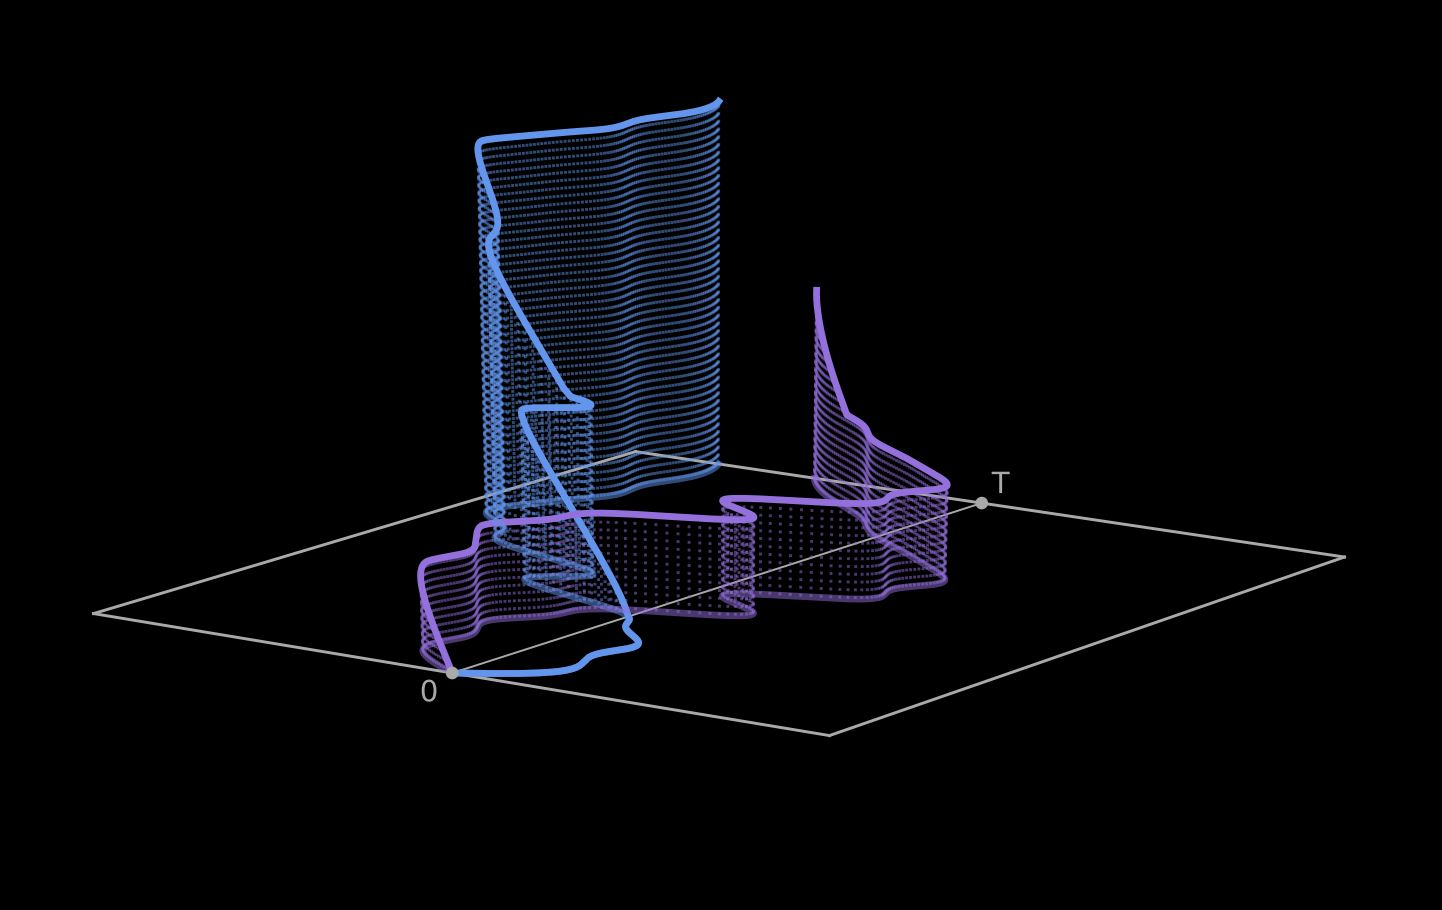
\includegraphics[scale =0.22]{KL/Figures/MaxDouble.JPG}
    %
    \label{fig:max3D}
\end{figure}



%========== Time Average and Integral ===========%
\begin{example} \label{ex:timeIntAvg}
 Consider  the time integral and average of a Brownian path, 
$y_t = 
f(X_t) = \int_0^t x_s\, ds, \ \bar{y}_{t}= 
\bar{f}(X_t) = \frac{1}{t}f(X_t). $
These are clearly centered processes and their covariance kernels of can be found explicitly. Starting with $Y$, 
$$\kappa_{Y}(s,t) =  \left(\int_0^s x_r dr,\int_0^t x_u du \right)_{L^2(\Q)} \overset{\textnormal{Fubini}}{=} \int_0^s\int_0^t \kappa_X(r,u) dr du.$$
A straightforward calculation gives
$\kappa_{Y}(s,t)  = \frac{s^2 t}{2} - \frac{s^3}{6}, \, s\le t.$
%\textbf{Moreover, it is straightforward to show that the eigenvalues are the square of the eigenvalues of Brownian (see Example \ref{ex:KLBM}).}
The covariance function of the time average follows immediately, namely
$\kappa_{\bar{Y}}(s,t)   = \frac{s}{2} -\frac{s^2}{6t}.$
We display in  \Cref{fig:AvgK,fig:IntK} the covariance kernel (top) and first eigenfunctions (bottom) of $f$ and $\bar{f}$, respectively.
The dashed lines in the top panels  are the eigenfunctions of the original (Brownian) path. Note the wider range in the eigenfunctions $F_1,F_2$ for $\bar{f}(X)$ compared to the integrated path for small $t$.  This might come from the greater fluctuations of the time average at inception. 

\end{example}
%========== Maximum ===========%
\begin{example} Consider the running maximum  functional $y_t= 
f(X_t) = \max_{0 \le s \le t} x_s$.  \Cref{fig:max3D} provides an illustration in the $(t,X,Y)$ plane. The mean function is in this case non-zero and$-$using, e.g., the reflection principle$-$given by $\E^{\Q}[y_t] = \sqrt{\frac{2}{\pi} t}$. The covariance kernel admits an explicit yet complicated expression \cite{Benichou}, 
$$\kappa_Y(s,t) = \frac{s}{2} + \frac{\sqrt{s(t-s)}-2\sqrt{st} + t \arcsin(\sqrt{s/t})}{\pi}, \quad s \le t.$$
\Cref{fig:MaxK} displays the covariance kernel (top) and first eigenfunctions (bottom). The latter turns out to be quite close to the eigenfunctions of Brownian motion. 

\end{example}



\begin{figure}[t]%[H]
%\centering
\caption{Covariance kernels (top) and eigenfunctions (bottom).}
\vspace{-4mm}
\begin{subfigure}[b]{0.32\textwidth}
    \centering
    \caption{Time average}
    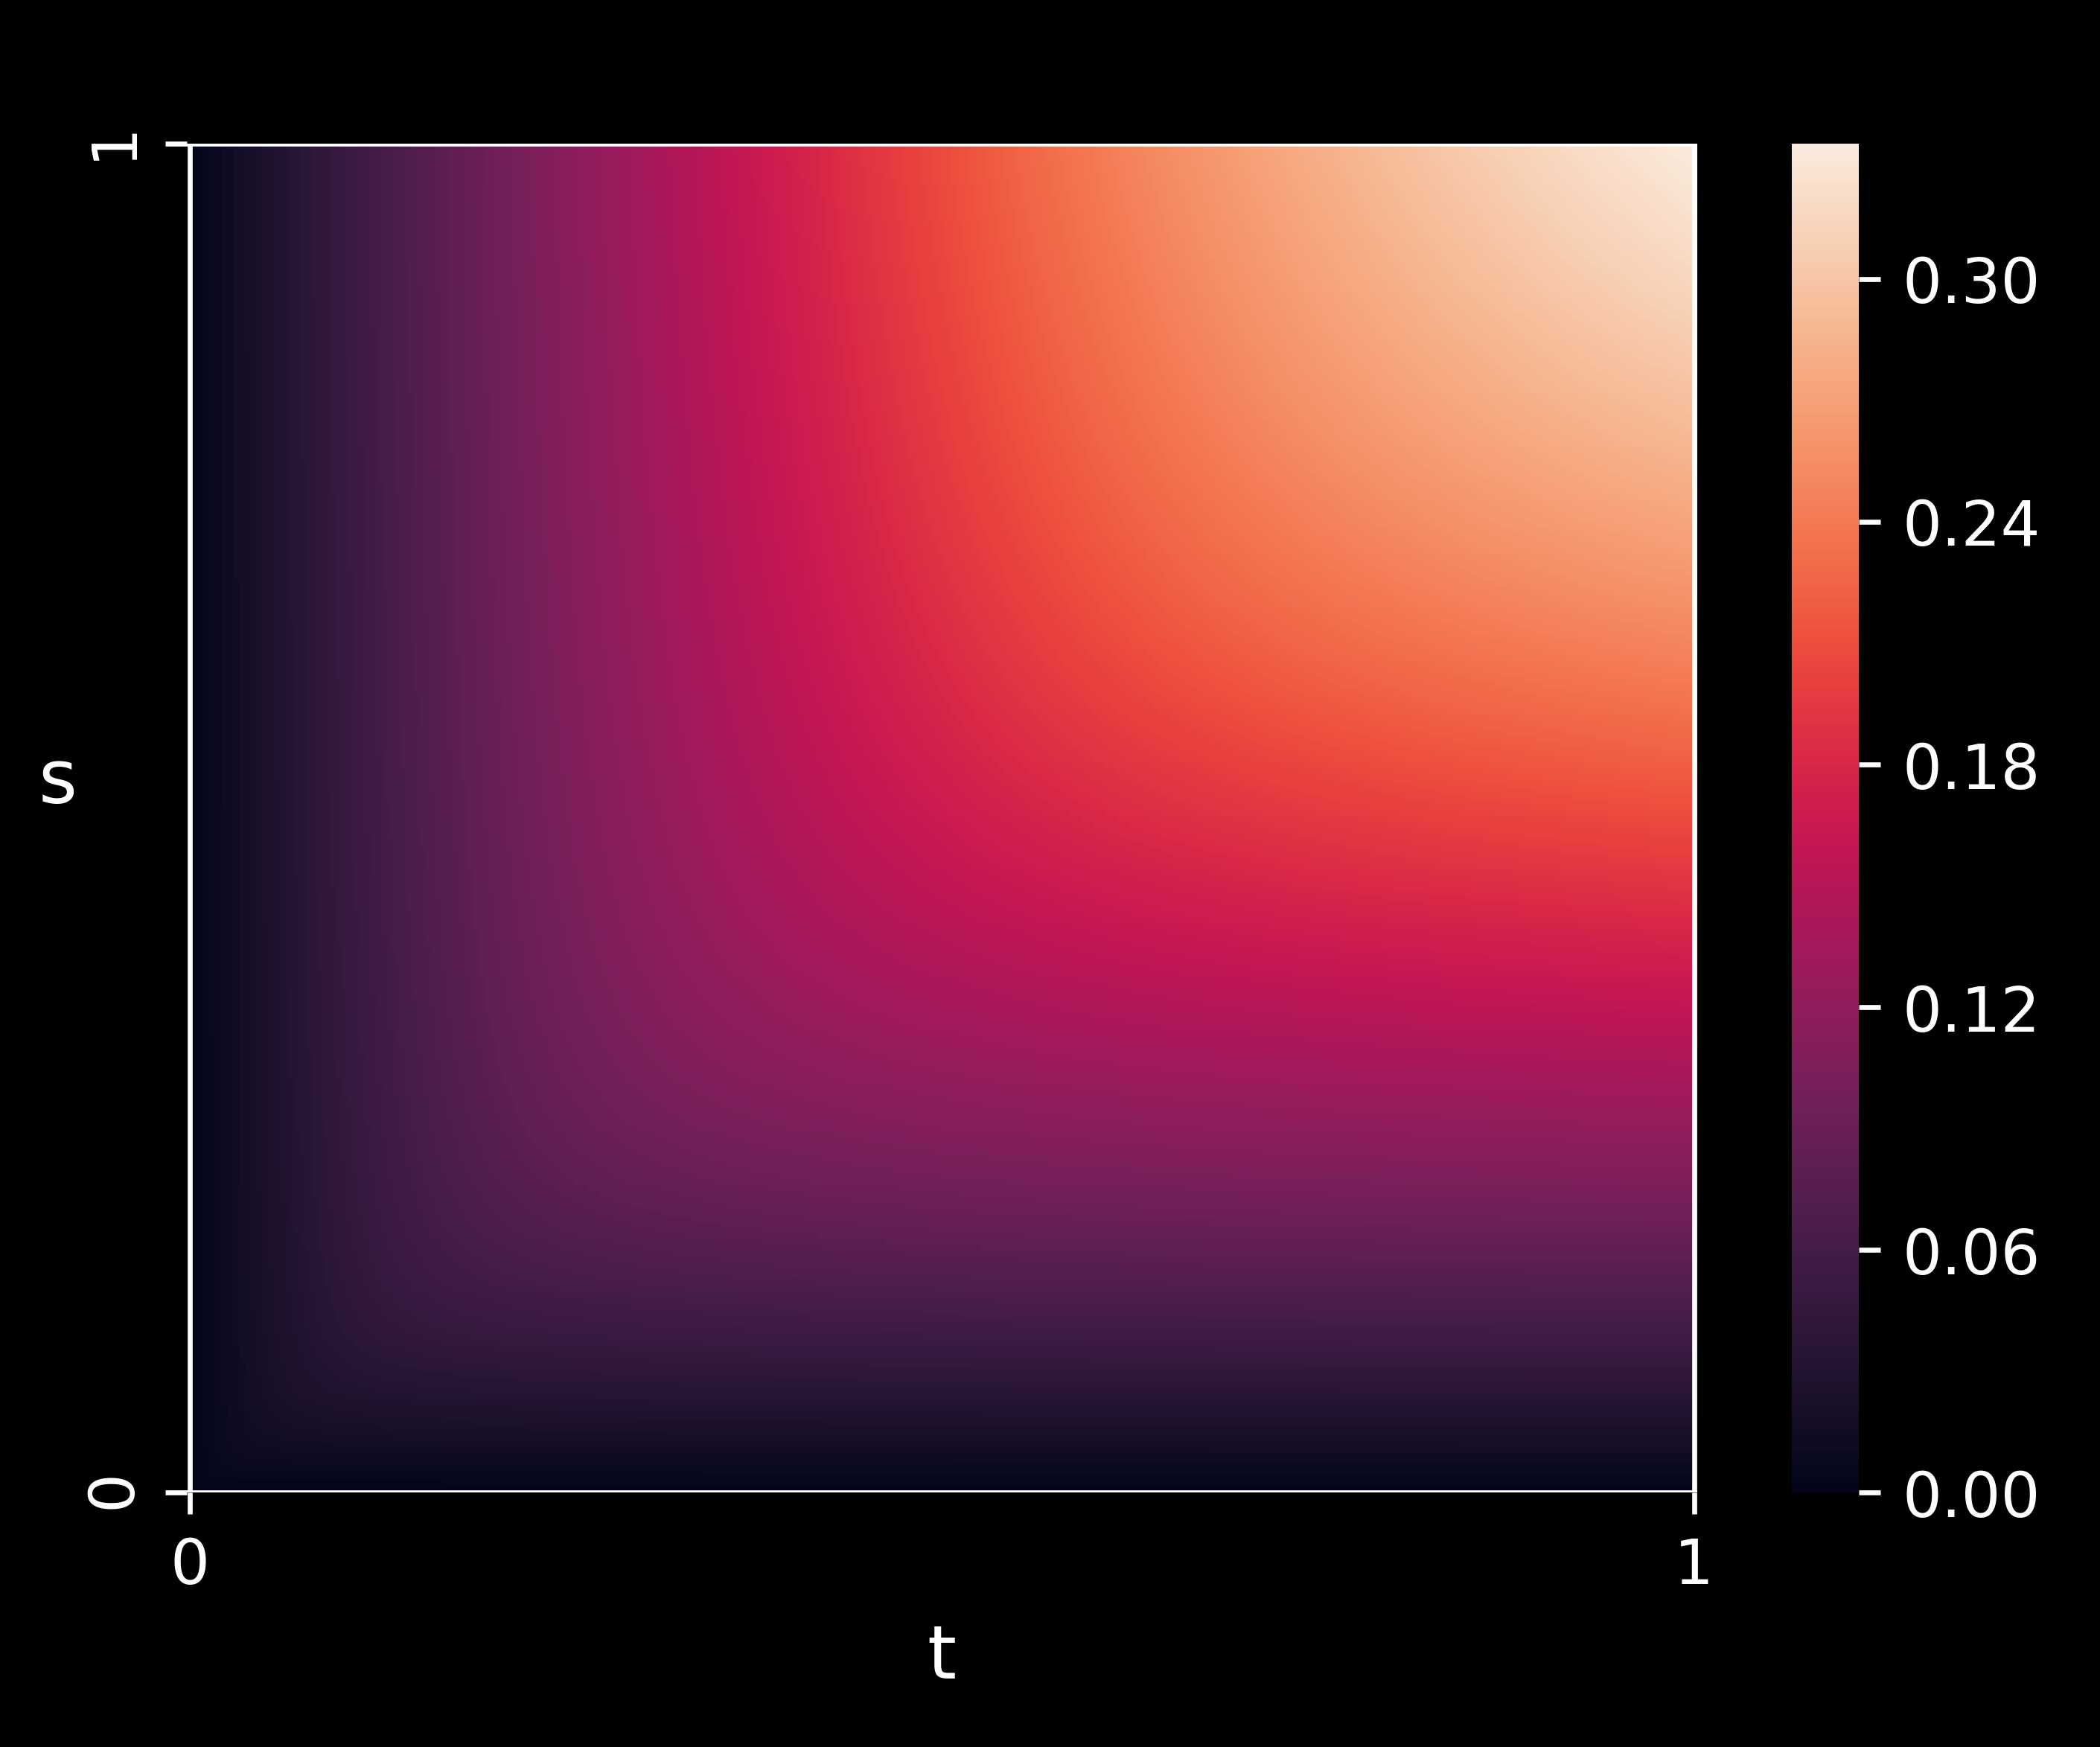
\includegraphics[scale =0.38]{KL/Figures/KLAverageKernel.png}
    \label{fig:AvgK}
\end{subfigure}
\begin{subfigure}[b]{0.32\textwidth}
    \centering
    \caption{Time integral}
    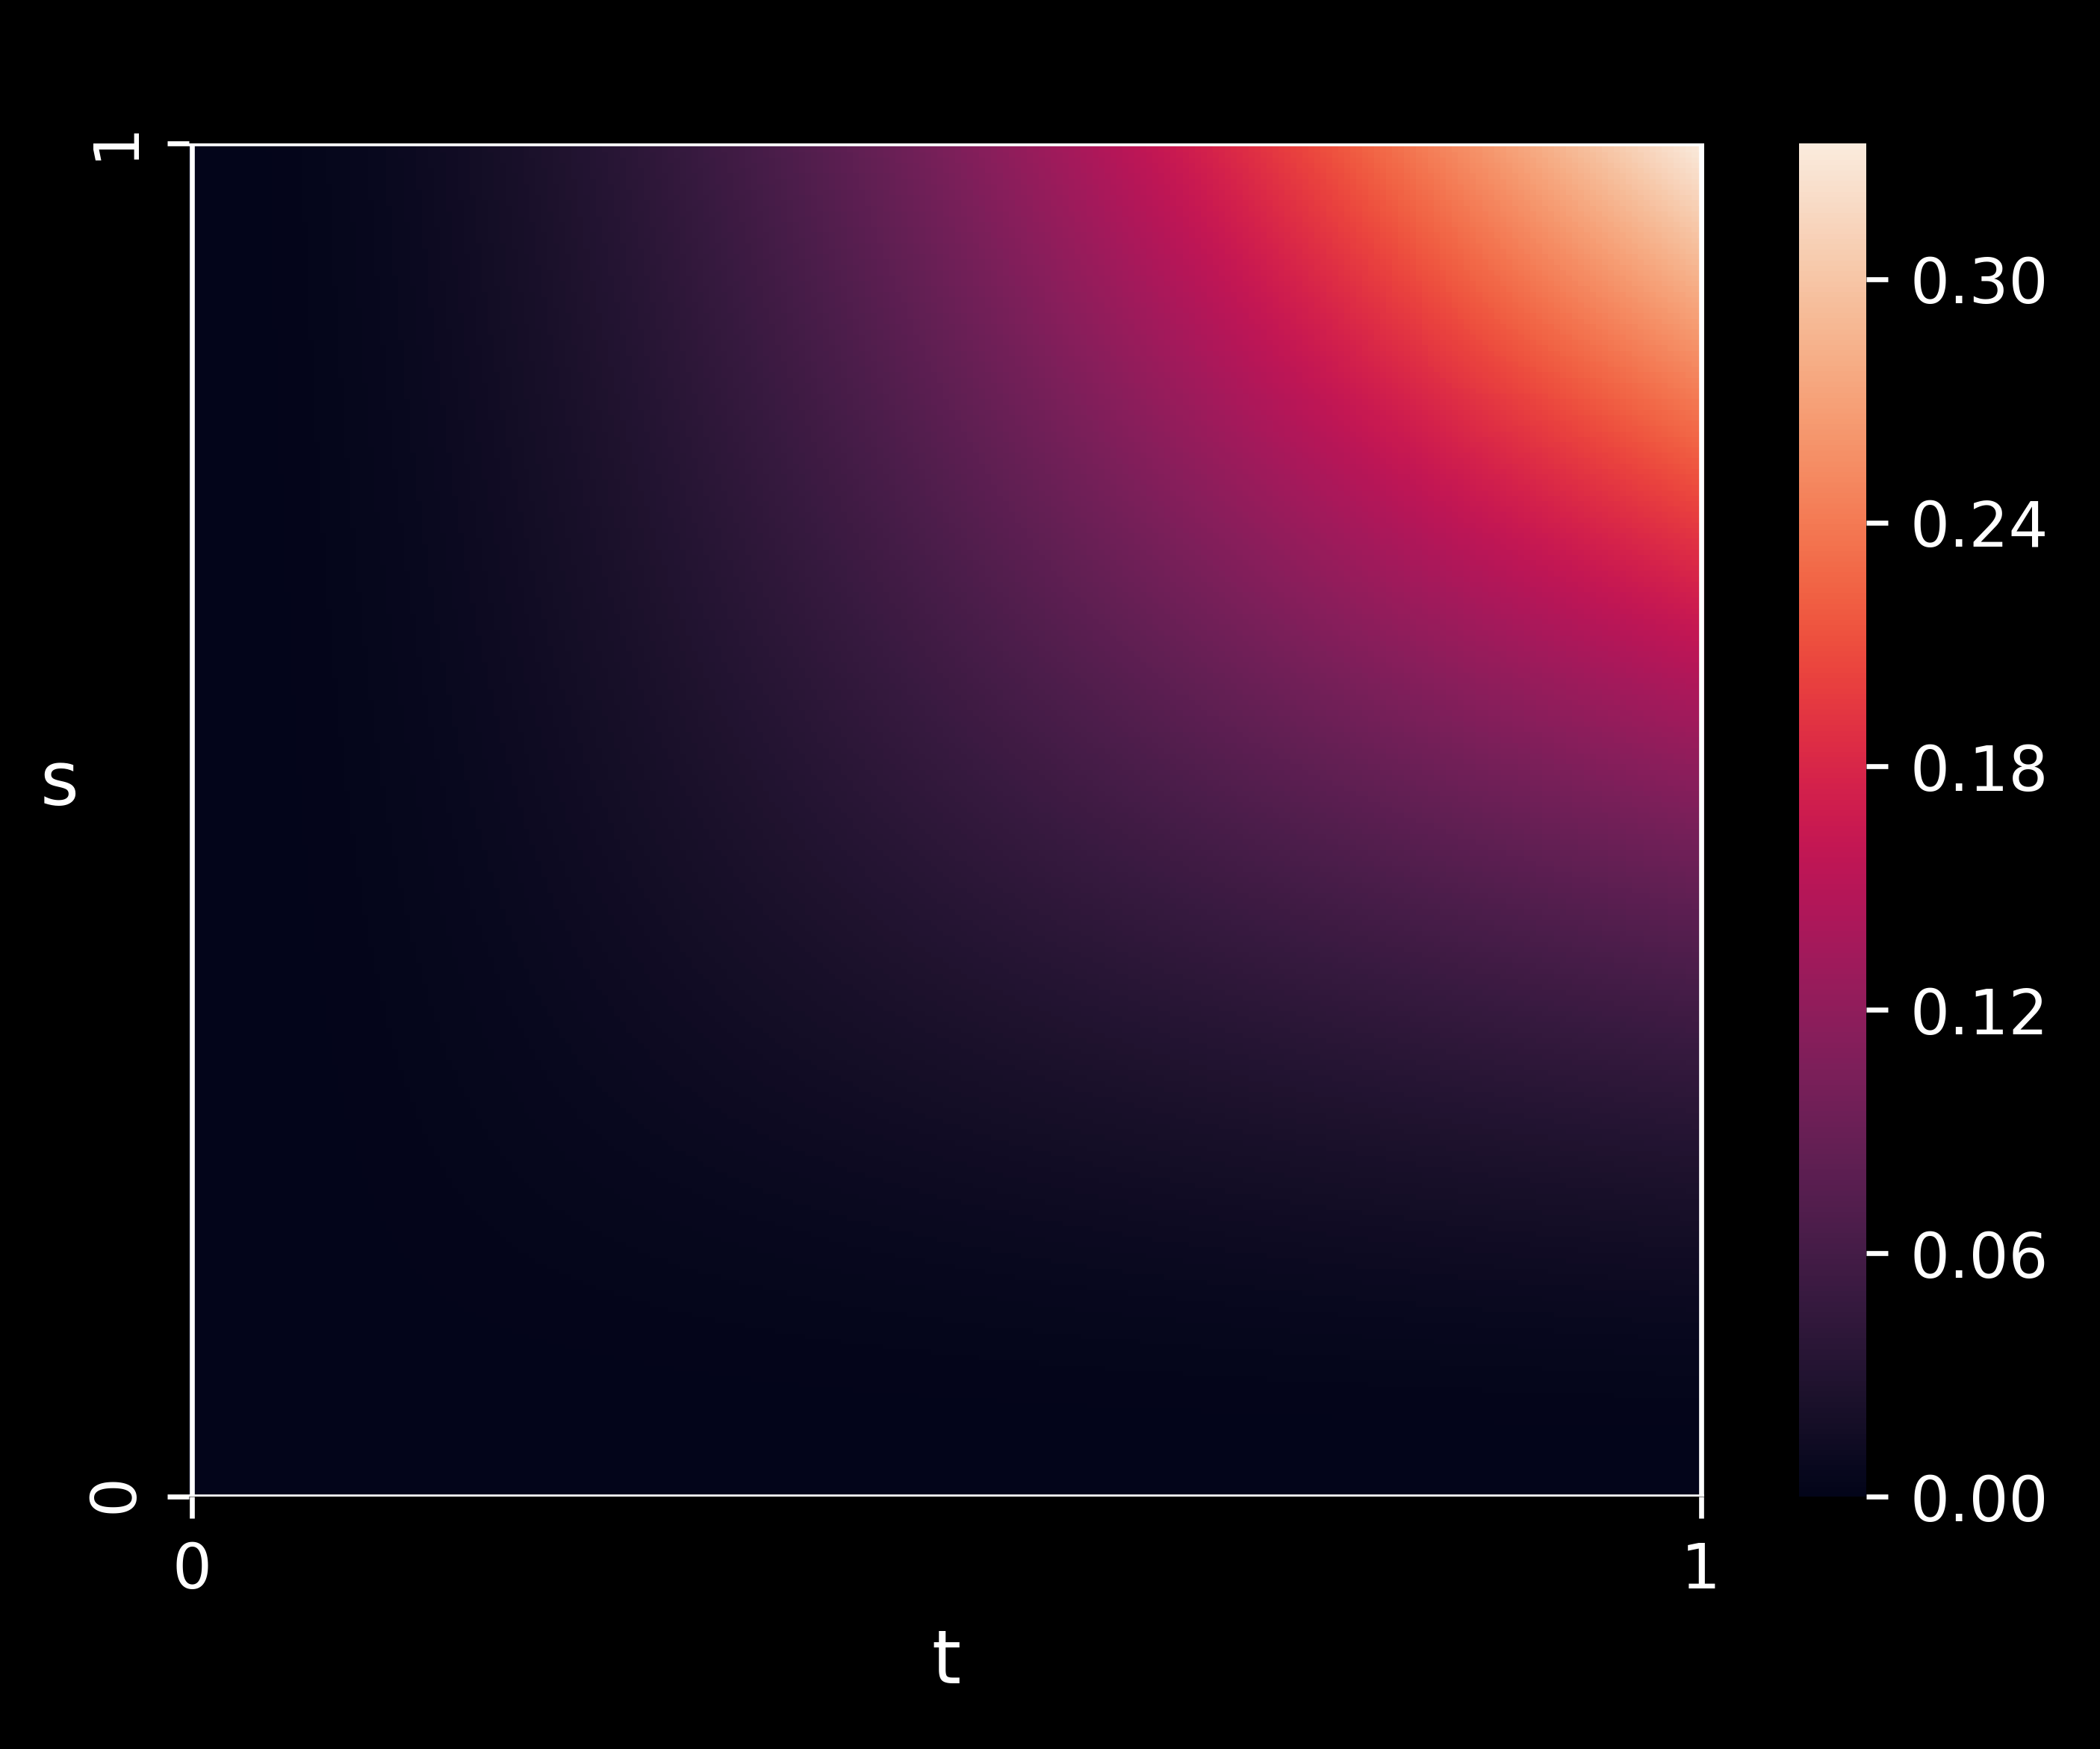
\includegraphics[scale =0.38]{KL/Figures/KLIntegralKernel.png}
    \label{fig:IntK}
\end{subfigure}
\begin{subfigure}[b]{0.32\textwidth}
    \centering
    \caption{Running maximum}
    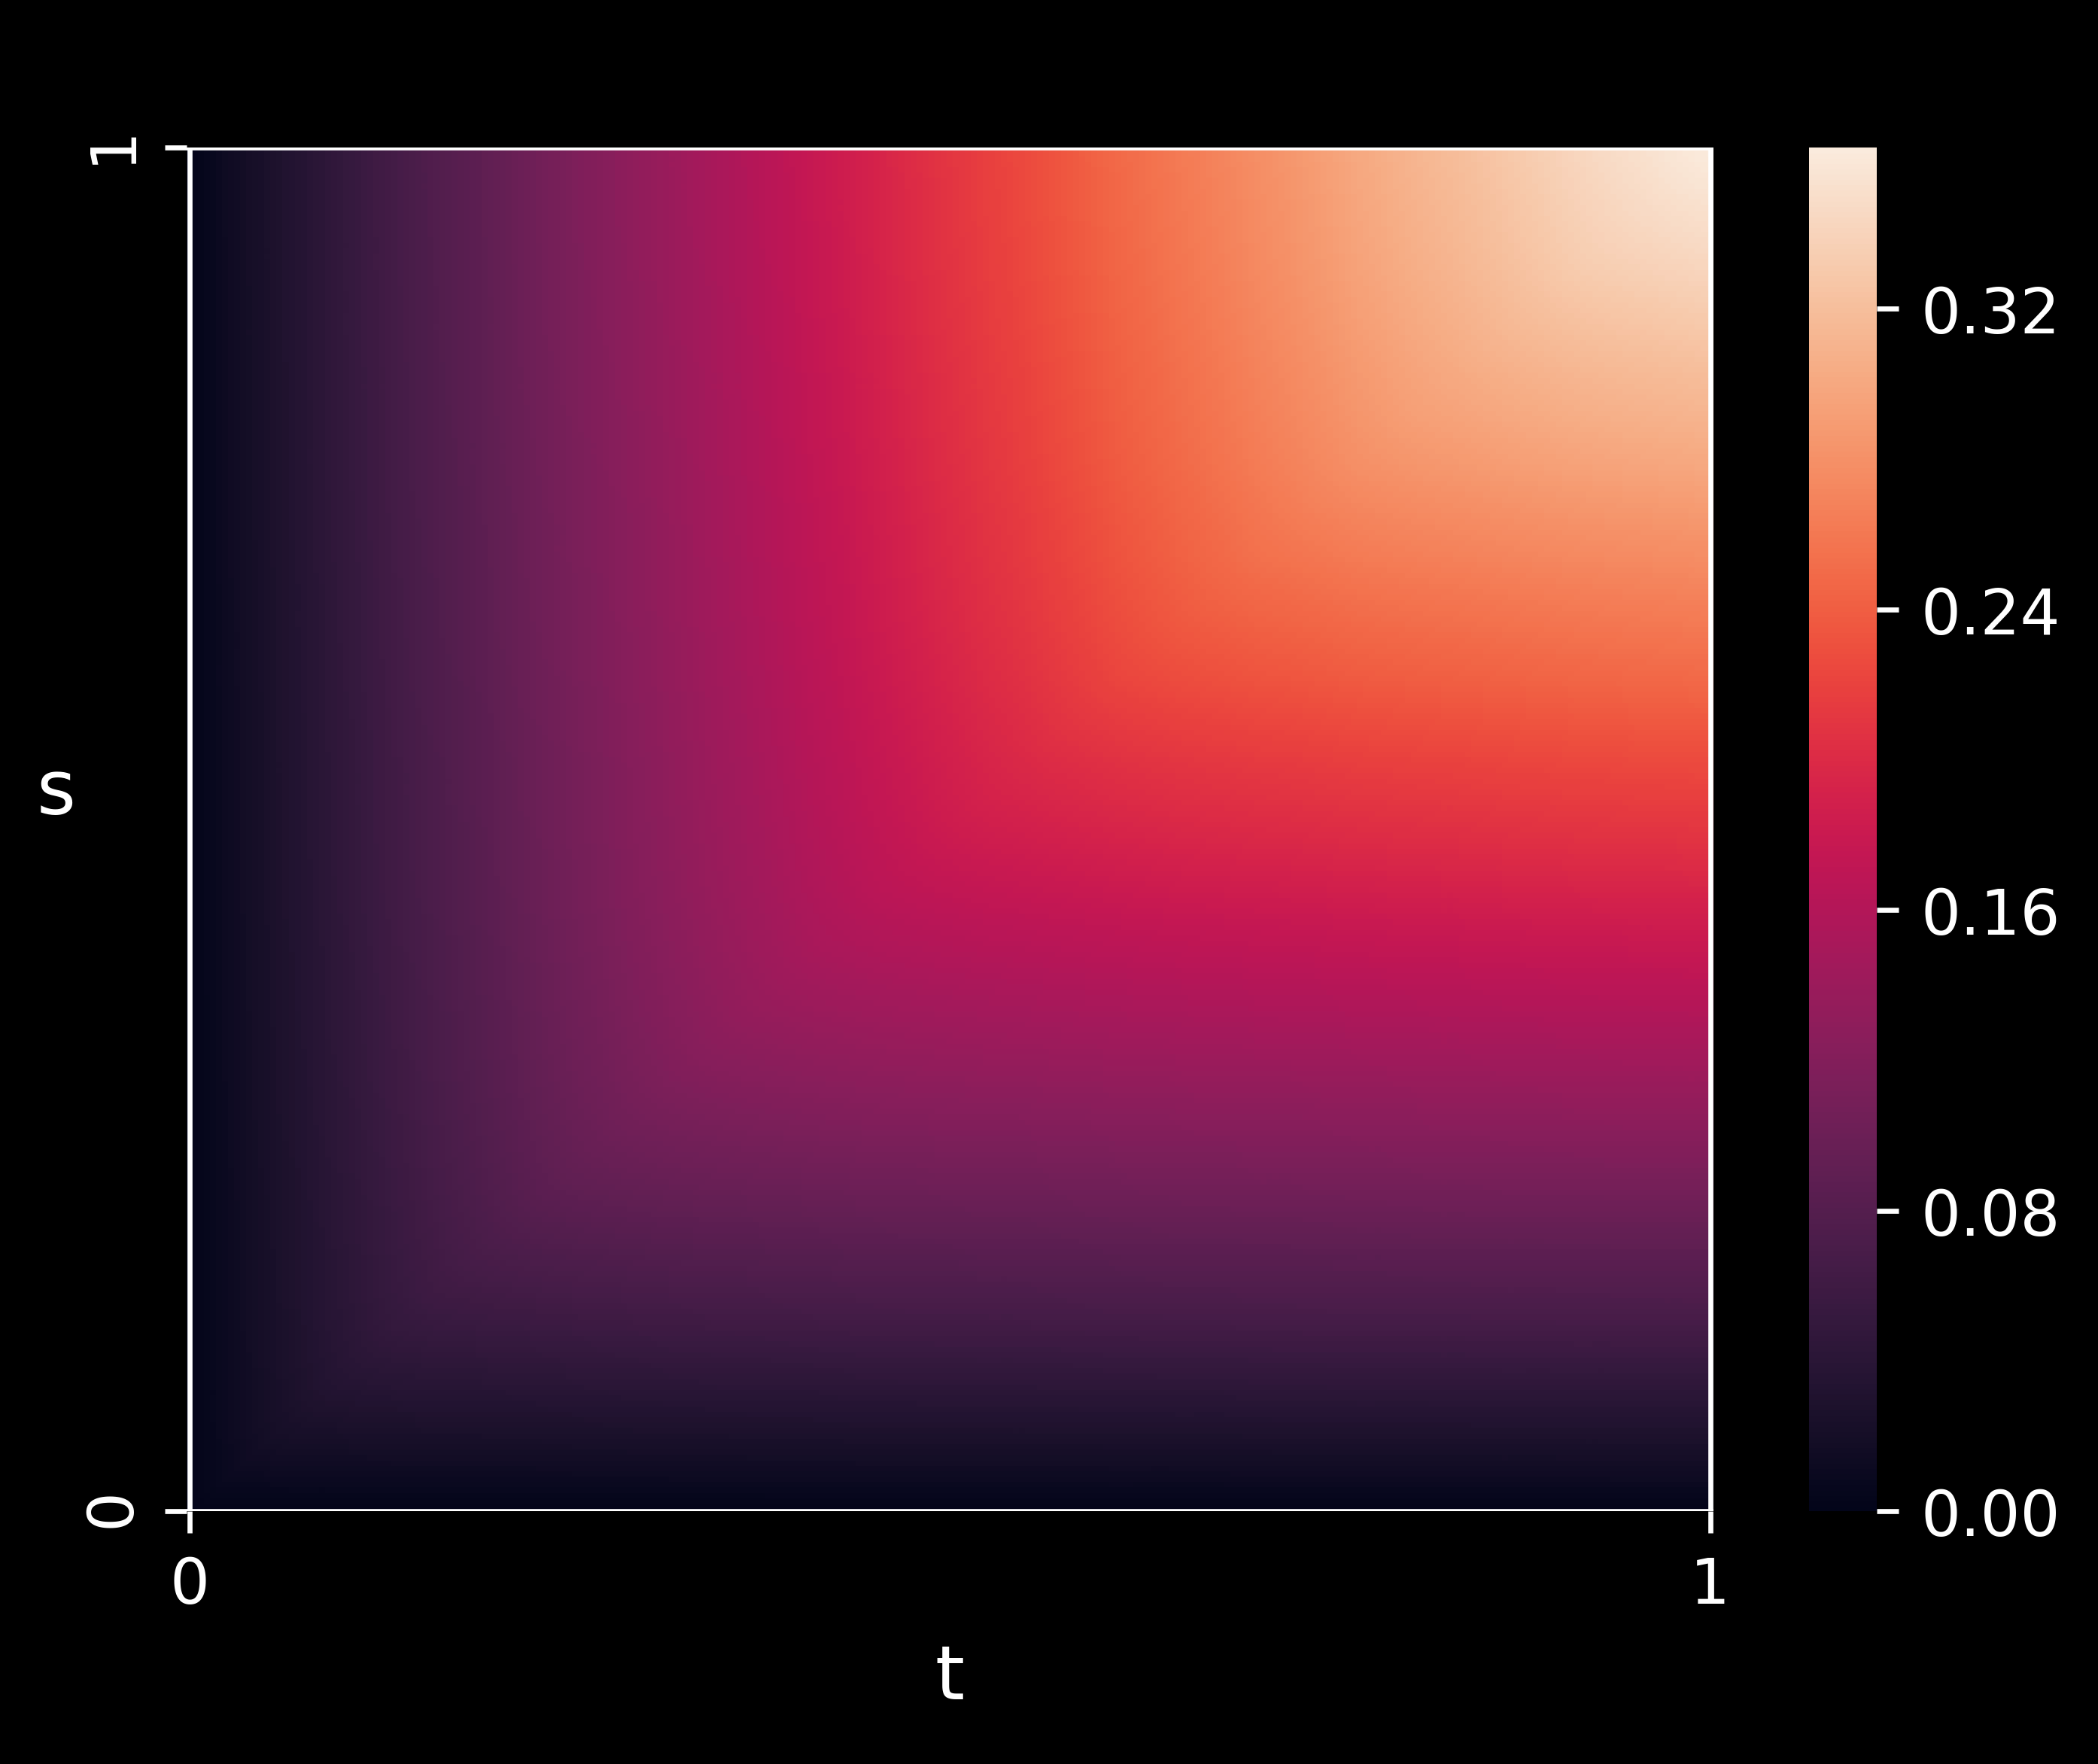
\includegraphics[scale =0.38]{KL/Figures/KLMaximumKernel.png}
    \label{fig:MaxK}
\end{subfigure}
\vspace{2mm}

%\centering
\begin{subfigure}[b]{0.32\textwidth}
    \centering
    %\caption{Time average}
    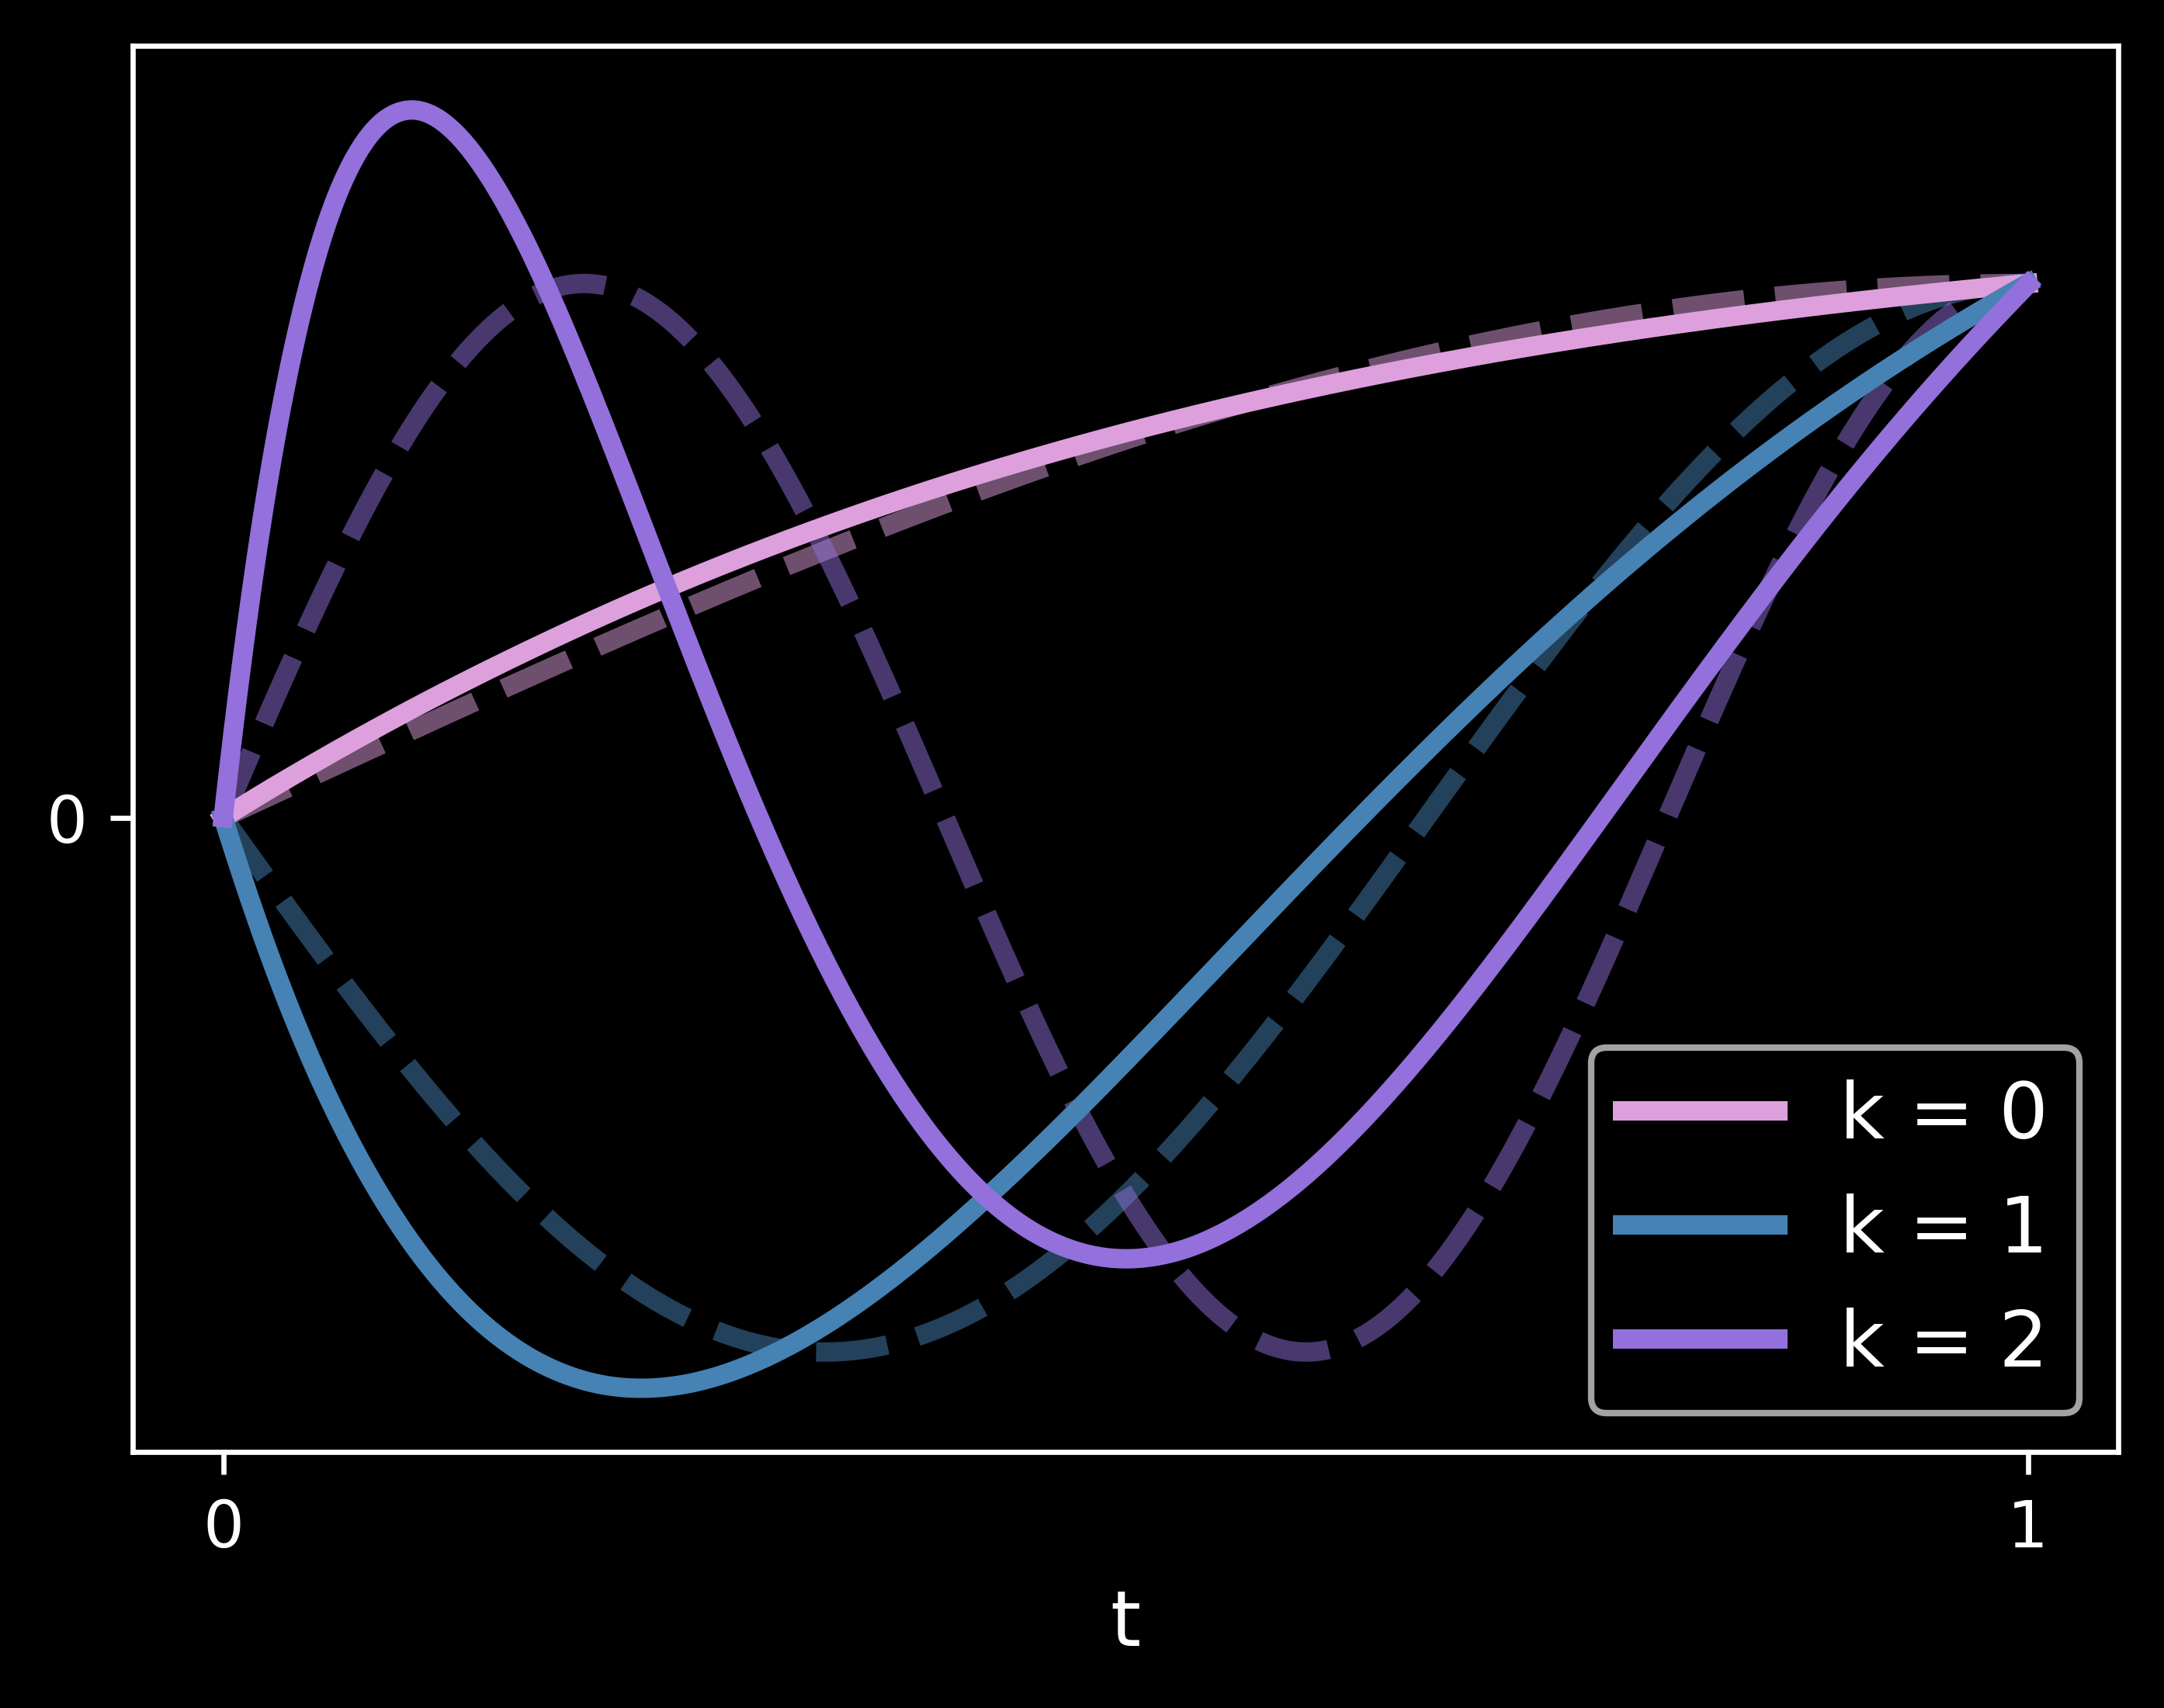
\includegraphics[scale =0.385]{KL/Figures/KLAsian.png}
\end{subfigure}
\begin{subfigure}[b]{0.32\textwidth}
    \centering
    %\caption{Time integral}
    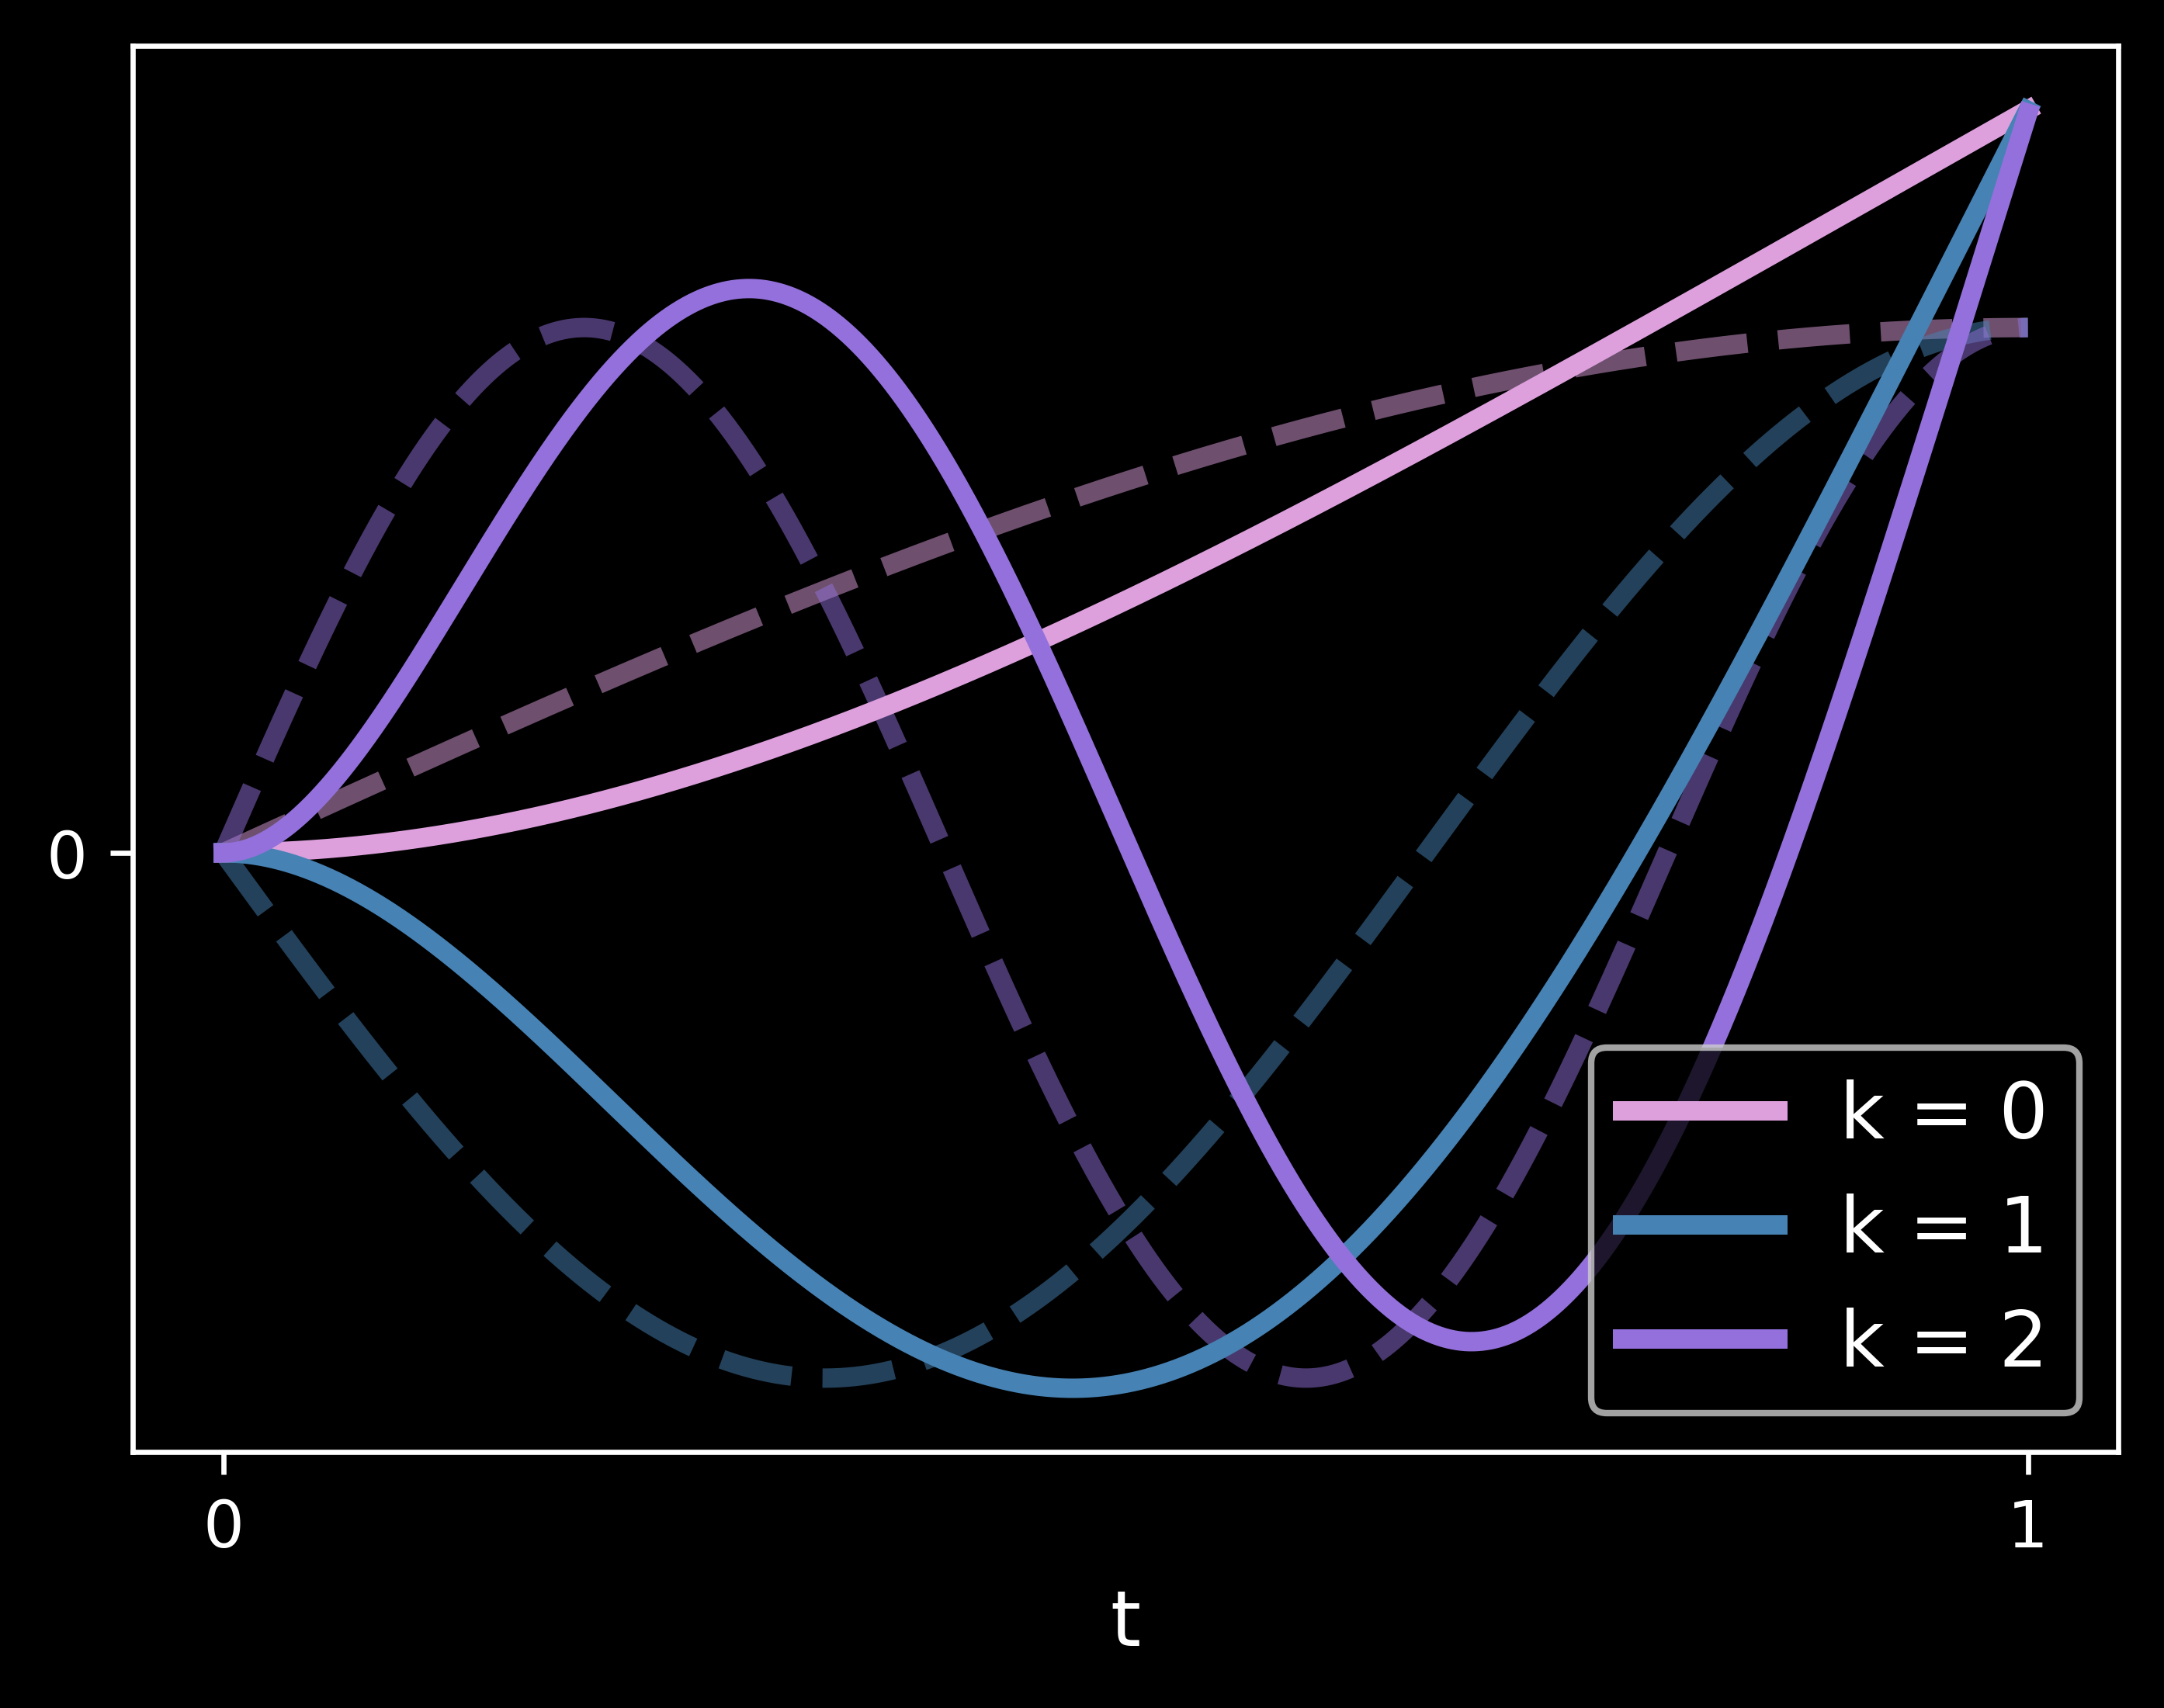
\includegraphics[scale =0.385]{KL/Figures/KLIntegral.png}
\end{subfigure}
\begin{subfigure}[b]{0.32\textwidth}
    \centering
    %\caption{Time integral}
    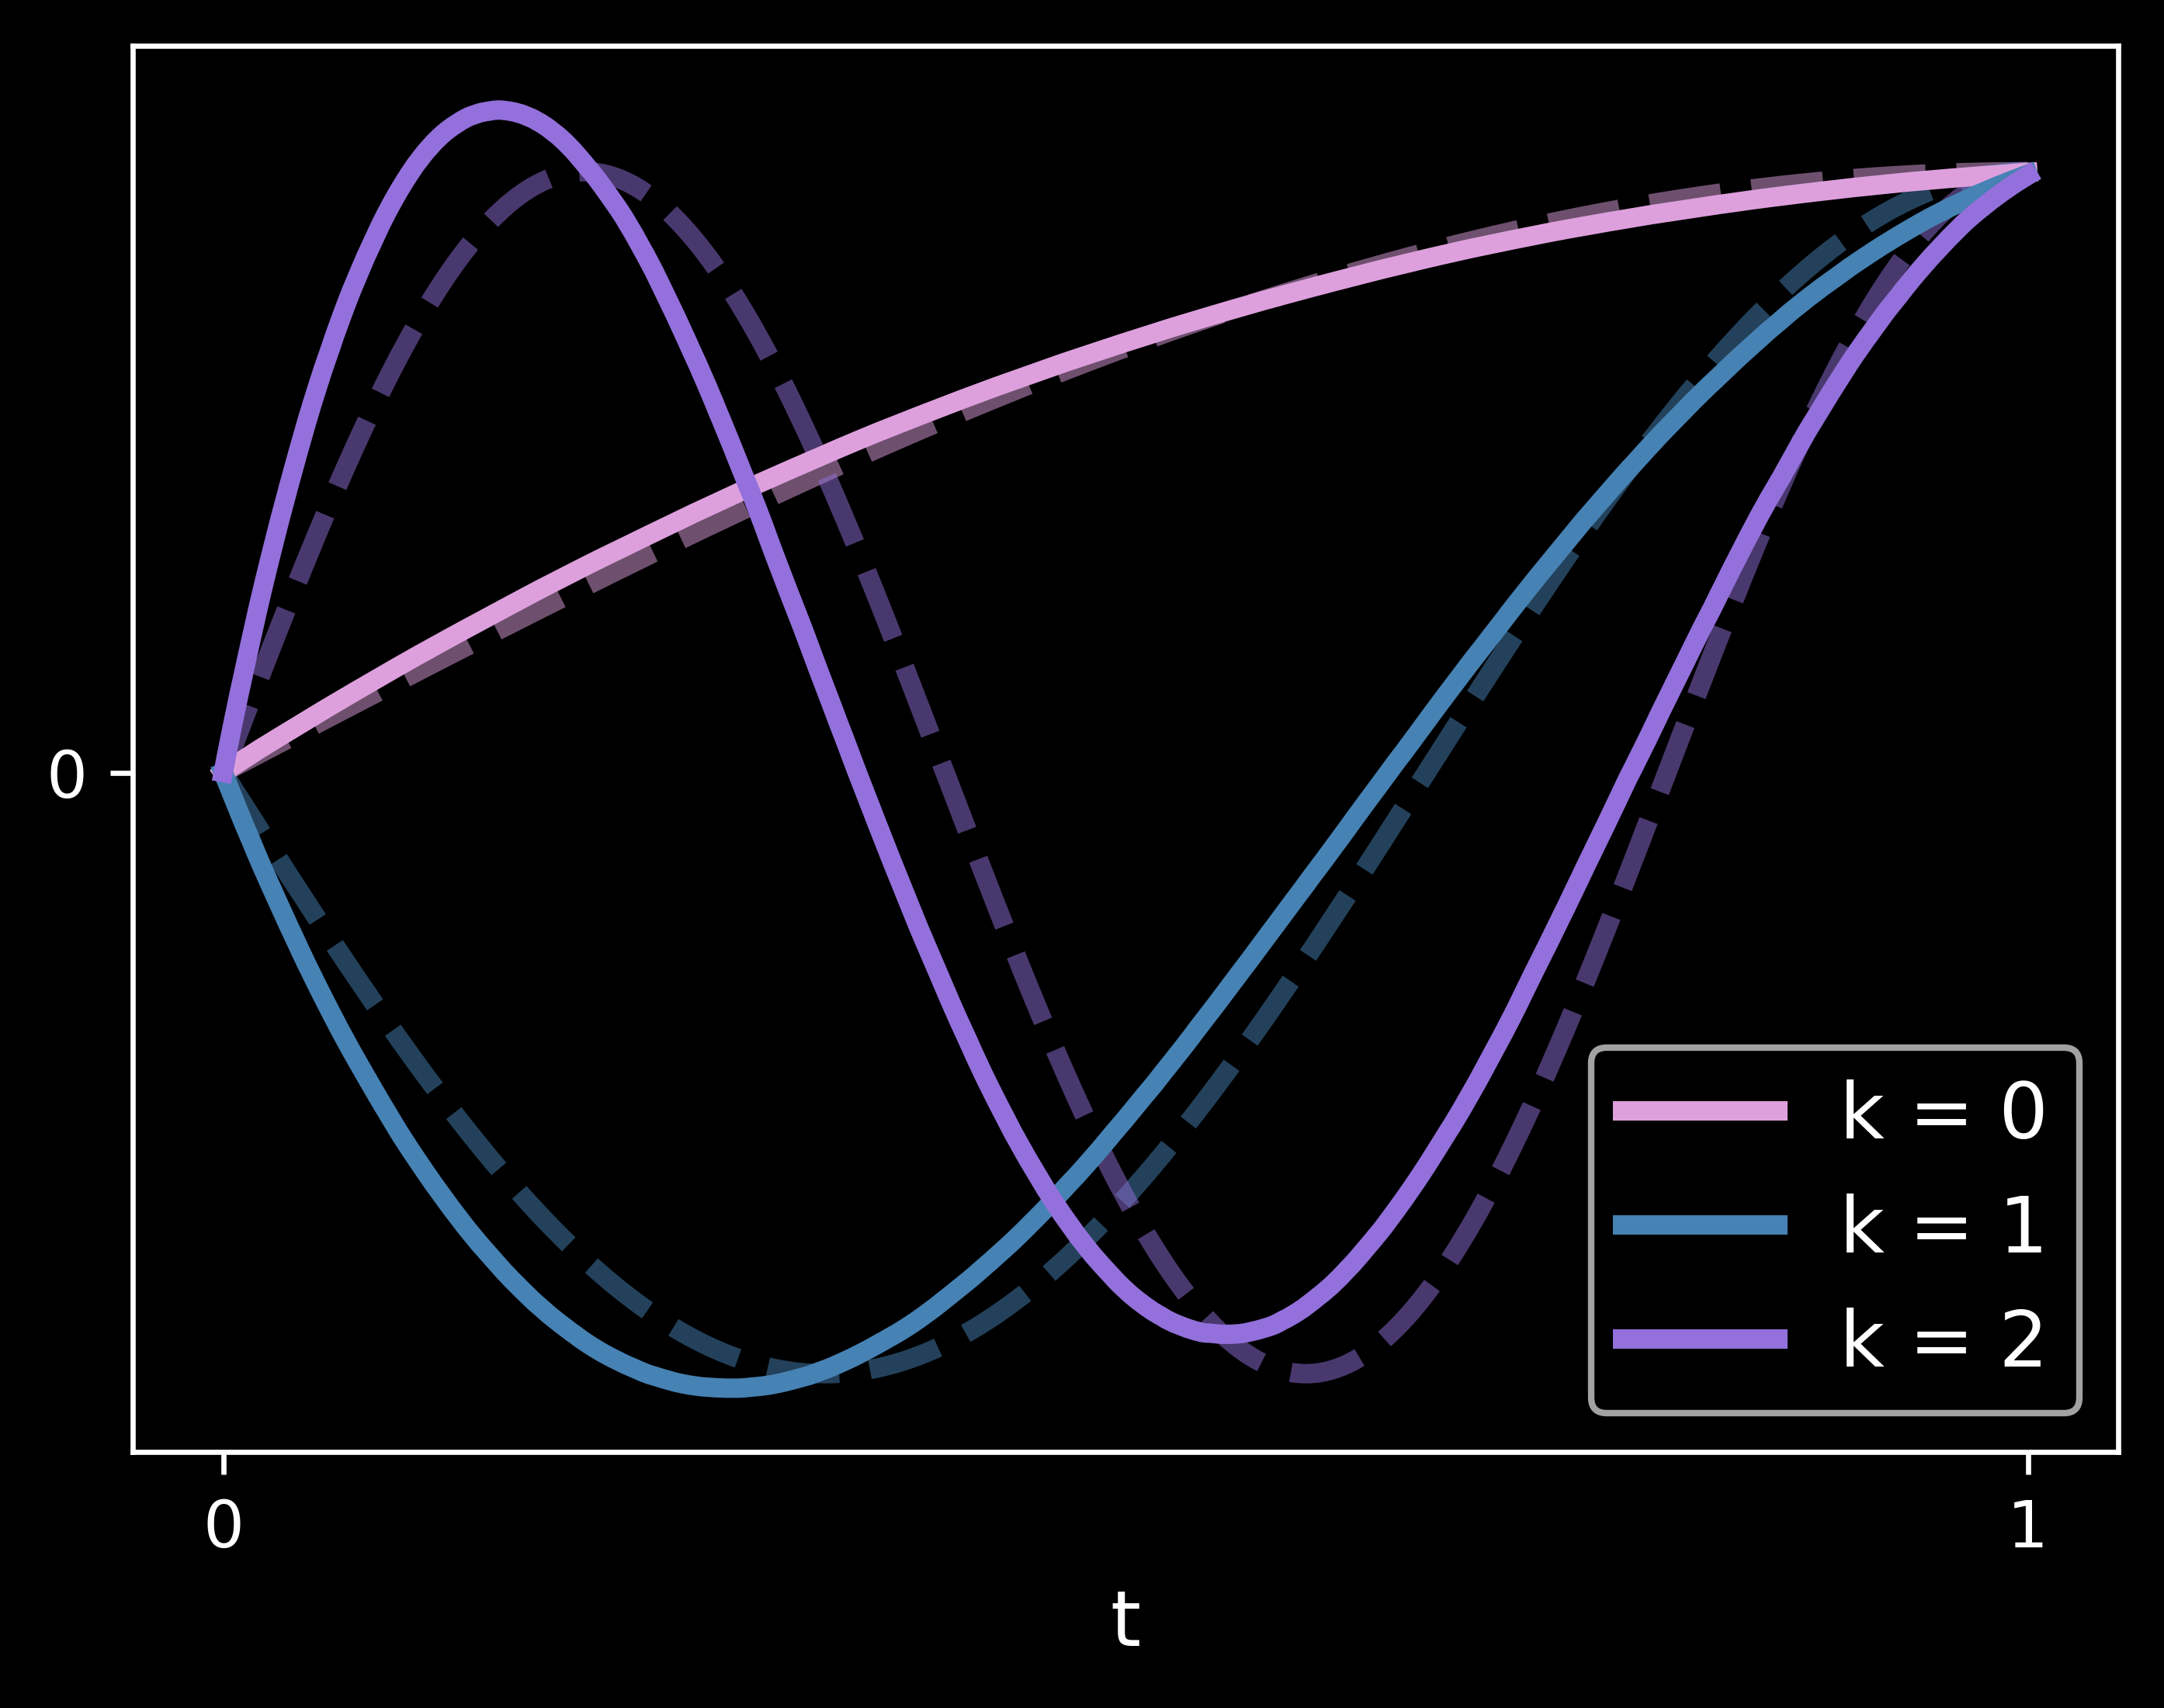
\includegraphics[scale =0.38]{KL/Figures/KLLookback.png}
\end{subfigure}
\vspace{1mm}
\begin{center}
    \footnotesize{
    \textit{Solid lines: transformed
     path.  Dashed lines: Brownian motion.}}
\end{center}
\vspace{-3mm}
\end{figure}
